\documentclass[border=2pt]{standalone}
\usepackage[T1]{fontenc}\usepackage{mathptmx}
\usepackage{amsmath,amssymb}\usepackage{tikz}\usepackage{pgfplots}
\pgfplotsset{compat=1.18}
\usetikzlibrary{shapes.geometric, arrows.meta, positioning, calc}
\setlength{\columnwidth}{3.45in}
\newcommand{\Pfree}{P_{\mathrm{free}}}\newcommand{\dfree}{d_{\mathrm{free}}}\newcommand{\pos}{\mathrm{pos}}
\newcommand{\ind}{\mathbf{1}}\newcommand{\Lin}{\mathcal{L}}
\pgfplotsset{ieeeplot/.style={width=\columnwidth, height=5.4cm,
 tick label style={font=\footnotesize}, label style={font=\footnotesize},
 legend style={font=\footnotesize, draw=black!60, fill=white, fill opacity=0.9, text opacity=1},
 grid=both, grid style={line width=0.2pt, draw=black!15}, major grid style={line width=0.3pt, draw=black!25},
 every axis plot/.append style={line width=0.8pt, mark size=2.2pt}}}
\begin{document}
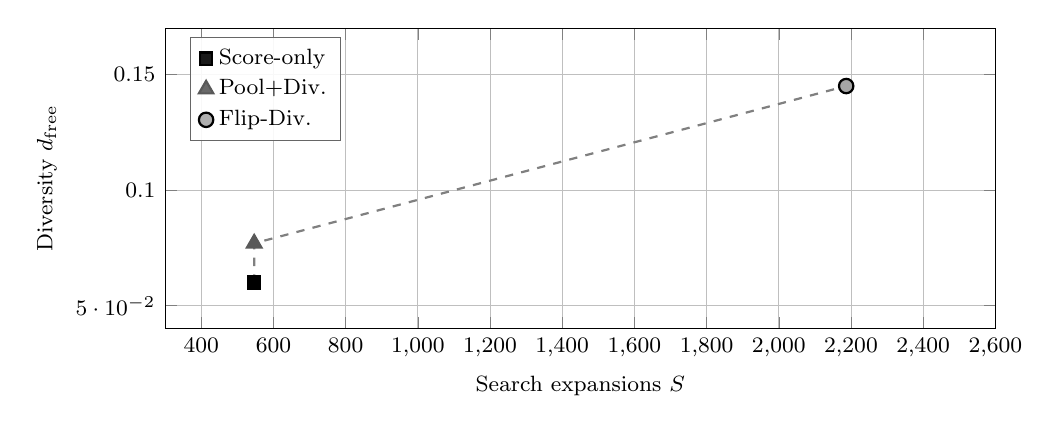
\begin{tikzpicture}
\begin{axis}[ieeeplot,
  xlabel={Search expansions $S$}, ylabel={Diversity $d_{\mathrm{free}}$},
  xmin=300, xmax=2600, ymin=0.04, ymax=0.17,
  legend pos=north west, legend cell align=left]
\addplot[black!50, dashed, forget plot] coordinates {(546.7,0.060) (546.7,0.077) (2186.7,0.145)};
\addplot[only marks, mark=square*, black] coordinates {(546.7,0.060)};
\addlegendentry{Score-only}
\addplot[only marks, mark=triangle*, black!65, mark size=3pt] coordinates {(546.7,0.077)};
\addlegendentry{Pool+Div.}
\addplot[only marks, mark=*, black!35, mark options={draw=black}, mark size=2.6pt] coordinates {(2186.7,0.145)};
\addlegendentry{Flip-Div.}
\end{axis}
\end{tikzpicture}
\end{document}
